\documentclass[aspectratio=169,10pt]{beamer}
\usepackage[utf8]{inputenc}
\usepackage{graphicx}
\usepackage{booktabs}
\usepackage{amsmath}
\graphicspath{{figures/}{../report/figures/}}
\usetheme{default}
\usecolortheme{seahorse}
\setbeamertemplate{navigation symbols}{}
\setbeamertemplate{footline}{\hfill\insertframenumber\hspace{2mm}\vspace{1mm}}
\definecolor{accent}{RGB}{30,90,150}
\setbeamercolor{frametitle}{fg=accent}
\setbeamercolor{title}{fg=accent}
\setbeamercolor{itemize item}{fg=accent}
\newcommand{\logA}{\ensuremath{\log A}}

\title{Stiffness of resistant breast-cancer cells\\from AFM force--distance curves}
\subtitle{Frequentist, Bayesian and machine-learning analysis}
\author{Giacomo Moretti}
\institute{University of Milano-Bicocca}
\date{}

\begin{document}

\begin{frame}\titlepage\end{frame}

\begin{frame}{Question and data}
\begin{columns}[T]
\begin{column}{0.55\textwidth}
\textbf{Question.} Is the nucleus mechanically different from the cytoplasm in resistant breast-cancer cells, and does it differ between lines?\medskip

\textbf{Data (JPK force files).}
\begin{itemize}
\item 257 curves, 4 groups: MCF7R / T47DR $\times$ cytoplasm / nucleus (55, 60, 59, 83)
\item cantilever MLCT-BIO; 1 session per line (25/02 and 18/03)
\item extend segment $\to$ mechanics; retract segment $\to$ adhesion
\item ``good curves'' pre-selected by the lab: no defective curves available
\end{itemize}
\end{column}
\begin{column}{0.42\textwidth}
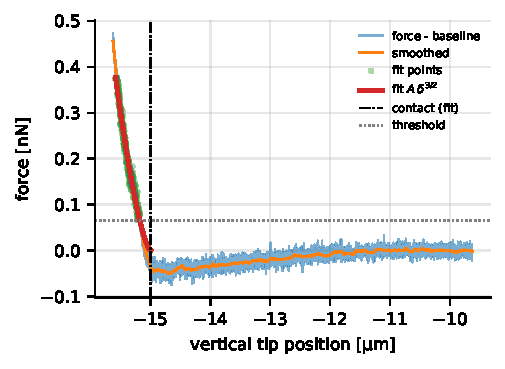
\includegraphics[width=\textwidth]{fit_example.pdf}
\vspace{-1mm}

{\footnotesize Baseline-corrected curve, contact point and Hertz-like fit.}
\end{column}
\end{columns}
\end{frame}

\begin{frame}{From curves to one number}
\begin{columns}[T]
\begin{column}{0.55\textwidth}
\begin{itemize}
\item robust linear baseline on the first 30\% of the curve
\item contact point from a threshold, then refitted
\item Hertz-like model with free contact point:
\[
F(\delta)=A\,\delta^{3/2},\qquad \delta=z_c-z
\]
\item $A$ = \textbf{effective} stiffness (nN\,$\mu$m$^{-3/2}$), \emph{not} Young's modulus: tip radius and Poisson ratio are missing
\item 9 preprocessing variants for systematics; median $R^2=0.986$
\item the analysis works on $\log A$ (skewed $A$)
\end{itemize}
\end{column}
\begin{column}{0.42\textwidth}
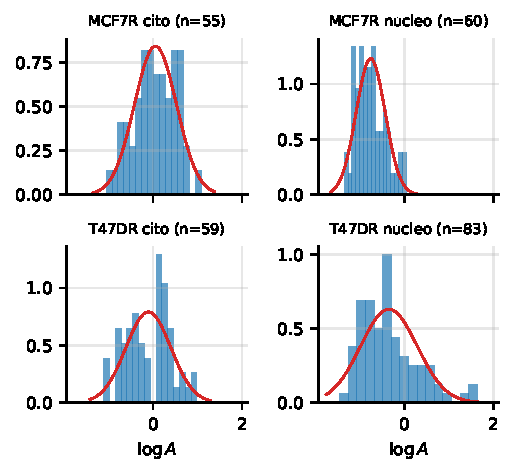
\includegraphics[width=\textwidth]{logA_groups.pdf}
\end{column}
\end{columns}
\end{frame}

\begin{frame}{Pipeline: ten notebooks, one repository}
\small
\begin{tabular}{@{}ll@{}}
\toprule
01 & JPK reading, CSV export, diagnostic QC (nothing discarded)\\
02 & baseline, contact point, Hertz-like fit, 9 variants\\
03 & frequentist: profile likelihood, toy MC, Holm, systematics\\
04 & Bayesian: MCMC, Bayes factors, priors, hierarchical, low statistics\\
05 & ML: anomaly detection (injected defects), classification, mixtures\\
06 & curve-shape ML: PCA, clustering, conformal prediction\\
07 & depth-resolved stiffness, fixed-force check, T47DR shape signal\\
08 & acquisition time, bursts of curves, temporal drift\\
09 & calibration between sessions, repeatability, preconditioning\\
10 & one Bayesian model: region, drift, position, burst\\
\bottomrule
\end{tabular}

\medskip
Notebooks 03--10 run from the tracked tables in \texttt{results/}; raw data are not in the repository.
\end{frame}

\begin{frame}{First result: the nucleus is softer ($\Delta=\mu_{nucleus}-\mu_{cytoplasm}$ in $\log A$)}
\begin{columns}[T]
\begin{column}{0.52\textwidth}
\centering
\small
\resizebox{\textwidth}{!}{\begin{tabular}{lcc}
\toprule
 & MCF7R & T47DR\\
\midrule
$n$ (cyto / nuc) & 55 / 60 & 59 / 83\\
$\Delta$ (68\%) & $-0.81\,(-0.89,-0.74)$ & $-0.25\,(-0.34,-0.15)$\\
ratio of $A$ & 0.44 & 0.78\\
$p$ (Wilks) & $<10^{-15}$ & 0.011\\
$\log_{10}BF_{10}$ & 13.9 & 0.6\\
\bottomrule
\end{tabular}}

\medskip
\raggedright
\begin{itemize}
\item toy MC: unbiased, pull width 0.98--1.00, 68\% coverage, size 5\%
\item 80\% power needs $|\Delta|\gtrsim0.22$--0.25: T47DR sits at the limit
\item $p\simeq0.01$ but Bayes factor only $\sim4{:}1$ for T47DR
\end{itemize}
\end{column}
\begin{column}{0.48\textwidth}
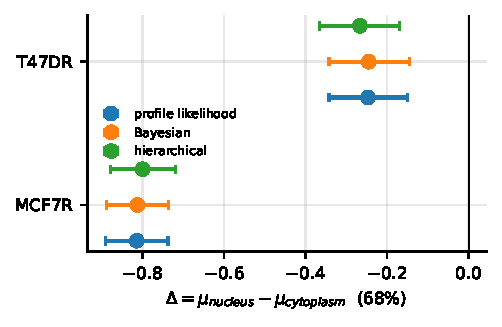
\includegraphics[width=\textwidth]{delta_methods.pdf}

{\footnotesize Three methods agree: profile likelihood, Bayesian, hierarchical.}
\end{column}
\end{columns}
\end{frame}

\begin{frame}{Validation of the statistics}
\begin{columns}[T]
\begin{column}{0.48\textwidth}
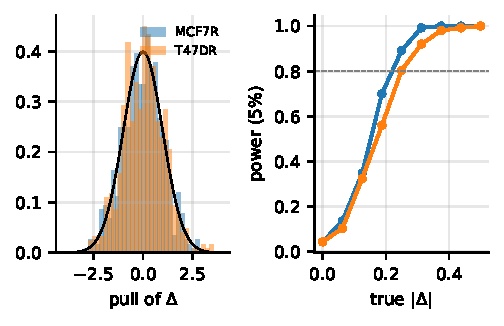
\includegraphics[width=\textwidth]{toys.pdf}

{\footnotesize Toy MC: pulls and power of the Wilks test.}
\end{column}
\begin{column}{0.48\textwidth}
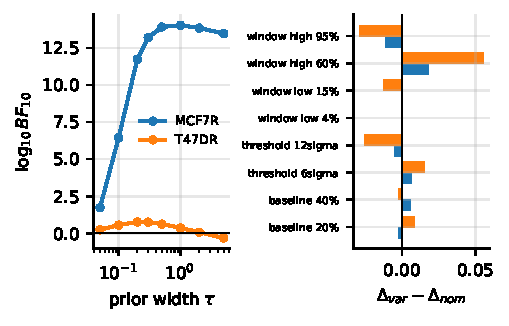
\includegraphics[width=\textwidth]{bf_systematics.pdf}

{\footnotesize Bayes factor vs prior width; preprocessing systematics.}
\end{column}
\end{columns}
\smallskip
\begin{itemize}
\item systematics (9 variants, Barlow criterion) $\le0.07$ in $\Delta$, below the statistical error
\item Student-$t$ not preferred; posterior predictive check shows skewness in the nucleus groups
\end{itemize}
\end{frame}

\begin{frame}{Machine learning}
\begin{columns}[T]
\begin{column}{0.55\textwidth}
\begin{itemize}
\item \textbf{Anomaly detection} on 1000 synthetic curves with 5 injected defects: Isolation Forest / robust Mahalanobis, AUC 0.88 / 0.87; weak on \texttt{wrong\_slope} (10--30\%)
\item \textbf{Region classifier:} AUC 0.95 (MCF7R), 0.63 (T47DR); transfers across lines
\item \textbf{Curve shape:} in T47DR the shape alone gives AUC 0.76; it is the local exponent (nucleus 1.50 vs cytoplasm 1.43)
\item \textbf{Conformal prediction:} T47DR sets are ambiguous for most curves
\end{itemize}
\end{column}
\begin{column}{0.43\textwidth}
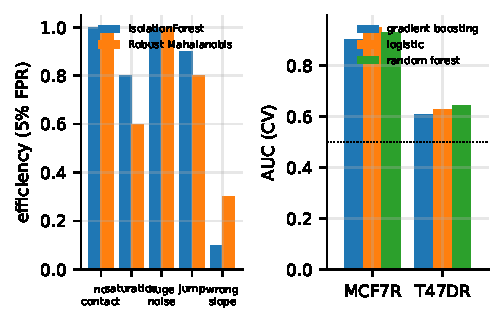
\includegraphics[width=0.85\textwidth]{ml.pdf}

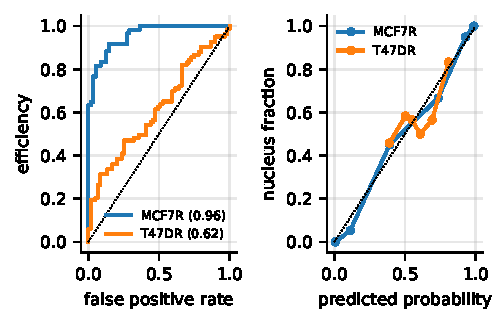
\includegraphics[width=0.85\textwidth]{roc_calibration.pdf}
\end{column}
\end{columns}
\end{frame}

\begin{frame}{Stiffness without the Hertz fit}
\begin{itemize}
\item \textbf{Fixed indentation:} $\Delta\log F(300\,\text{nm})=-0.76$ (MCF7R), $-0.35$ (T47DR)
\item \textbf{Fixed force:} the nucleus needs a larger indentation: $\times1.7$ (MCF7R), $+0.15$ to $+0.19$ in log (T47DR)
\item the nucleus is softer at every depth between 50 and 600~nm
\item free exponent $\approx1.5$: the model is adequate on average
\end{itemize}
\medskip
\alert{But}: these checks do not remove confounding from the experimental design $\ldots$
\end{frame}

\begin{frame}{The design: regions measured in separate time blocks}
\begin{columns}[T]
\begin{column}{0.6\textwidth}
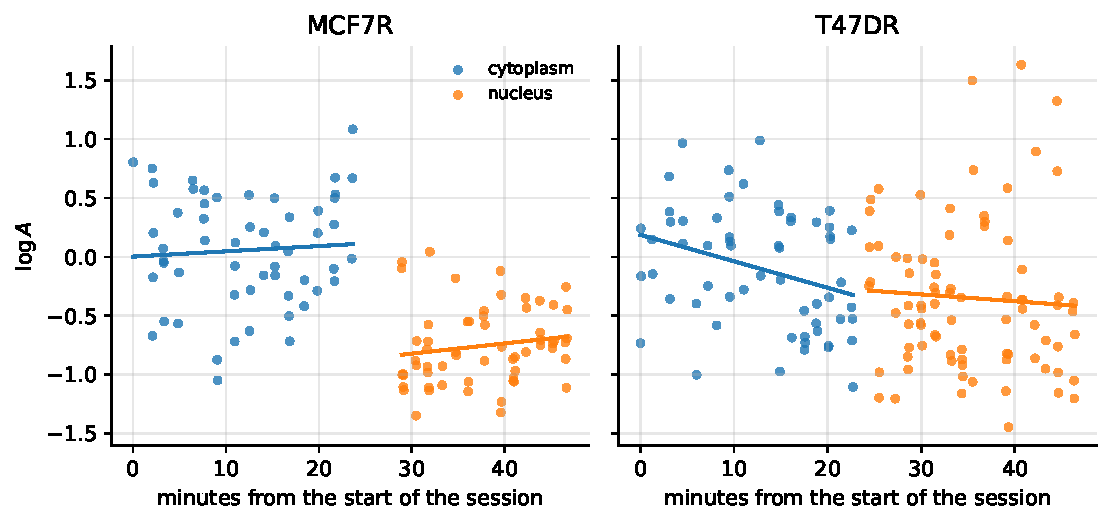
\includegraphics[width=\textwidth]{timeline.pdf}
\end{column}
\begin{column}{0.38\textwidth}
\begin{itemize}
\item JPK timestamps: in both sessions cytoplasm first (0--23 min), nucleus after (25--47 min), \emph{no overlap}
\item region $\equiv$ time block
\item T47DR: $\log A$ decreases during the session ($-0.13$ per 10 min); this drift alone predicts $\Delta\approx-0.30$
\item MCF7R: drift goes the opposite way, so the effect grows ($-0.97\pm0.17$)
\end{itemize}
\end{column}
\end{columns}
\end{frame}

\begin{frame}{Bursts, repeatability, preconditioning}
\begin{columns}[T]
\begin{column}{0.55\textwidth}
\begin{itemize}
\item curves come in \textbf{bursts} of 3--5 at the same spot (2 s apart); 13--17 bursts per group
\item intra-burst correlation moderate (ICC 0--0.18), design effect $\simeq1.4$; SE of $\Delta$ $+5\%$ / $+16\%$
\item repeatability sd $=0.33$--$0.61$ in $\log A$: scatter at one spot $\approx$ scatter between spots
\item \textbf{first curve at a spot is stiffer}: second $-$ first $=-0.25\pm0.09$ ($p=0.013$)
\item nucleus bursts are longer $\Rightarrow$ more softened curves in the nucleus mean
\item first curve only: $\Delta=-0.77\pm0.13$ (MCF7R), $-0.01\pm0.26$ (T47DR)
\end{itemize}
\end{column}
\begin{column}{0.42\textwidth}
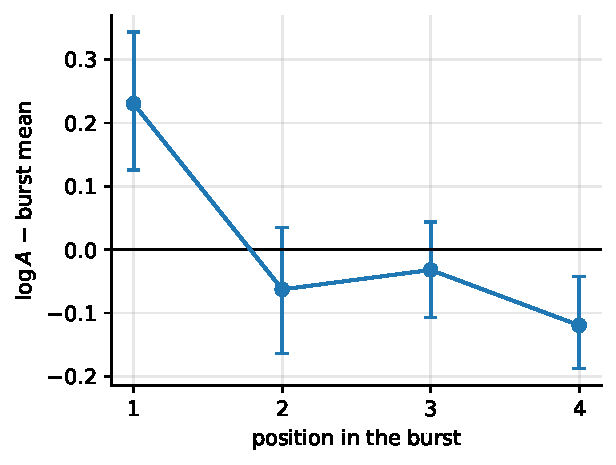
\includegraphics[width=\textwidth]{preconditioning.pdf}
\end{column}
\end{columns}
\end{frame}

\begin{frame}{Calibration differs between sessions}
\begin{columns}[T]
\begin{column}{0.5\textwidth}
\small
\begin{tabular}{lcc}
\toprule
 & 25/02 (MCF7R) & 18/03 (T47DR)\\
\midrule
cantilever & 2300FE & 2300FE\\
spring constant & 0.119 N/m & 0.080 N/m\\
sensitivity & 10.9 nm/V & 14.0 nm/V\\
force setpoint & 0.75 nN & 0.75 nN\\
\bottomrule
\end{tabular}
\end{column}
\begin{column}{0.48\textwidth}
\begin{itemize}
\item same cantilever, $-40\%$ in $k$: shifts $\ln A$ by up to 0.4
\item line differences ($-0.16$ cyto, $+0.41$ nucleus) cannot be interpreted, \textbf{not even in sign}
\item inside a session $k$ is common to both regions and cancels in $\Delta$
\end{itemize}
\end{column}
\end{columns}
\end{frame}

\begin{frame}{One model for all of this}
\[
y_i=a+\beta\,r_i+\gamma\,t_i+\delta_{p_i}+u_b+\varepsilon_i,\qquad u_b\sim\mathcal N(0,\tau^2)
\]
{\small region $r$, time $t$ (drift $\gamma$), position $p$ in the burst, burst effect $u_b$ integrated out; \texttt{emcee}}
\vspace{-1mm}
\begin{columns}[T]
\begin{column}{0.5\textwidth}
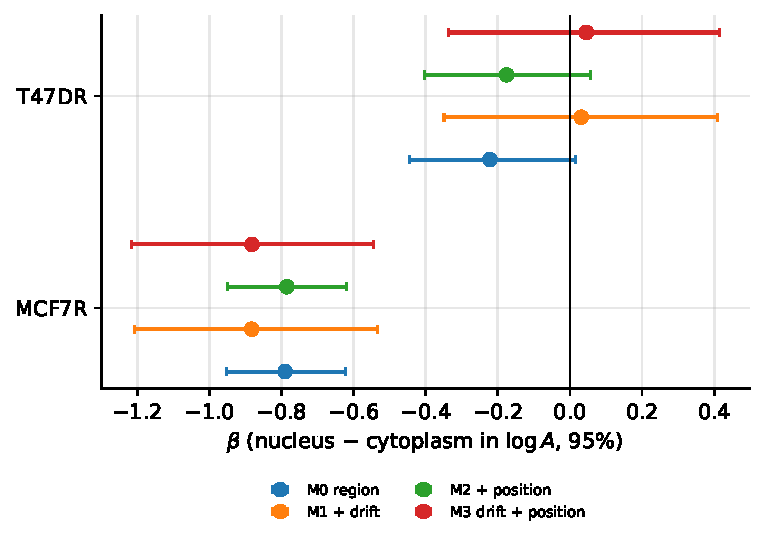
\includegraphics[width=\textwidth]{beta_models.pdf}
\end{column}
\begin{column}{0.48\textwidth}
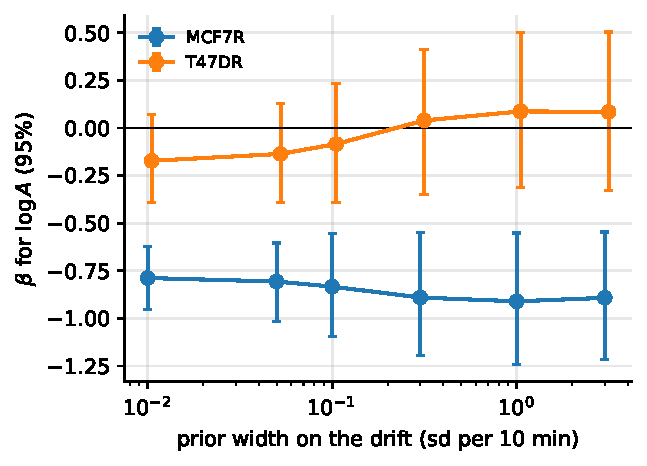
\includegraphics[width=\textwidth]{drift_sensitivity.pdf}
\end{column}
\end{columns}
\end{frame}

\begin{frame}{What survives}
\begin{columns}[T]
\begin{column}{0.48\textwidth}
\textbf{MCF7R: solid}
\begin{itemize}
\item $\beta=-0.79$ without drift, $-0.88$ with drift and position; 95\% $[-1.22,-0.55]$
\item same for force at fixed indentation
\item independent of the prior on the drift
\end{itemize}
\end{column}
\begin{column}{0.5\textwidth}
\textbf{T47DR: not established}
\begin{itemize}
\item stiffness: $\beta=-0.22\,[-0.45,+0.02]$ with bursts; $+0.03\,[-0.35,+0.41]$ with drift
\item $P(\beta<0)$ from 0.92 (negligible drift) to 0.34 (free drift)
\item \textbf{robust:} the nucleus has a higher contact-law exponent ($+0.062$, $[0.019,0.103]$)
\end{itemize}
\end{column}
\end{columns}
\medskip
Effect difference between lines: $\beta_{MCF7R}-\beta_{T47DR}=-0.93\,[-1.42,-0.43]$ (calibration-free, still confounded with the session).
\end{frame}

\begin{frame}{Limits and what would settle it}
\textbf{Limits}
\begin{itemize}
\item region $\equiv$ time block; line $\equiv$ session; calibration differs by 40\%
\item no cell identifier (bursts as a proxy); pre-selected curves; effective parameter, not Young's modulus
\end{itemize}
\bigskip
\textbf{Next measurements}
\begin{itemize}
\item cytoplasm and nucleus \textbf{alternated} on the same cells, with the cell identifier
\item calibration repeated within and between sessions
\item first curve at each spot (or fewer indentations per spot)
\item the ``bad'' curves, to validate anomaly detectors on real defects
\end{itemize}
\end{frame}

\begin{frame}{Summary}
\begin{itemize}
\item reproducible pipeline of 10 notebooks, results in a public repository (no raw data)
\item nucleus softer than cytoplasm in MCF7R: \textbf{robust} to drift, bursts, preconditioning and the fit model
\item T47DR: the stiffness difference is \textbf{not established}; a higher contact-law exponent in the nucleus is
\item the experimental design (time blocks, calibration, preconditioning) limits what these data can say
\end{itemize}
\bigskip
\centering
\footnotesize \texttt{github.com/gmoretti03/AFM}\quad $\cdot$\quad full report: \texttt{Docs/report/main.pdf}
\end{frame}

\end{document}
